\documentclass[12pt,a4paper]{article}
\usepackage[utf8]{inputenc}
\usepackage{amsmath}
\usepackage{amsfonts}
\usepackage{amssymb}
\usepackage{graphicx}
\begin{document}
%\pagenumbering{none}
\begin{titlepage}

	\begin{center}
		\begin{Huge}
			Tribhuvan University\\
			
\includegraphics[scale=1.6]{./Image/logo.png}\\
			Institute of Engineering\\
			Pulchowk Campus\\[1.6cm]		
		\end{Huge}
		\textbf{A\\
		Project On\\
		USB Oscilloscope}\\[1cm]
		\textbf{Submitted To:}\\
		Department of\\
		Electronics and Computer\\Engineering\\[1.6cm]
	
		\textbf{Submitted By:}\\
		Prajjwal Raj Kandel (068BEX428)\\
		Prakash Gautam (068Bex429)\\
		Sudip Prasai (068BEX442)\\
		Utsav Bhetwal (068BEX447)\\[.3cm]
		\textbf{\small{May 22, 2014}}	
	\end{center}	
\end{titlepage}
\vfill
\newpage
\pagenumbering{roman}

\tableofcontents
\vfill
\newpage
\pagenumbering{arabic}
\abstract{We have proposed to build a USB oscilloscope that will present the electronic signals on the display units of computer and the data read will be allowed to be saved on text files and may even be exported to excel or any other spreadsheet application. We will use a high speed ADC to initially convert the analog electrical signal into digital signal and the data will be sent to the PC via the USB port. The data read by the PC will then be displayed graphically in the program written in C++. We will use our own graph plotter application to present the read data. }
\newpage
\section{Introduction}
One of the most frequent experiments students and researchers would do, working on study of electrical signals is to trace out the waveform of the signal as a function of time. This is done very successfully by a Oscilloscope. But the price that is attached with an Oscilloscope of a reasonable performance is beyond reach of many students. \\

In context of countries like Nepal, schools and colleges check their budget twice before even thinking of buying a new oscilloscope, let alone the curious students like us who can't even think of it.\\

But since computers have been vastly cheap and almost every student has a computer now, it makes sense to use the computational power of a computer to do the job of oscilloscope borrowing the help of computer screen to trace the electrical signals.\\

Our project is based upon the same idea of making oscilloscope assuming the availability of computer with relative ease than an oscilloscope. Furthermore parents would rather buy a multipurpose computer than an oscilloscope where they can't use Facebook on.\\

Additional small aid box beside that computer making it function as an oscilloscope would sound extremely great.\\

\section{Objectives}
As a part of syllabus of IOE, students of III${}^{rd}$ yr II${}^{nd}$ part are required to carry out a mini project. This project of ours is primarily intended for the fulfillment of the same. But we are committed to make this project not \emph{just another project}, we are expecting some real usefulness beside completing the requirement together with learning basic hardware electronics coupled with software interface.\\

We hope to learn a great deal of electronics on the application level.\\

Some of the objectives can be listed as:\\
\begin{enumerate}
\item To fulfill the course requirement.
\item To learn software and hardware integration on real scale
\item To create easily affordable oscilloscope for students.
\end{enumerate}

\section{Methodology}


\subsection{Sensing}
First the input signal will be converted into Digital signal with a high speed ADC. If the frequency of input signal is $f$ and $n$ samples are taken per cycle of the signal then the frequency of sampling will be:
\begin{equation}
	\textit{Sampling Frequency}= f*n
\end{equation}
Owing to Nyquist criterion the value of $n$  should be greater than $2$ but this will not suffice to generate smooth signal so we will need $n\geq 100$.\\

If we restrict ourselves with the input frequency of the order of hundred of kilo hertz then. The sampling frequency should be around
\begin{eqnarray*}
 \textit{Sampling Frequency}&=&100K*100\\
 &=& 10MHz\\
\end{eqnarray*}

So we would require ADC with the output time less than $10^{-7}s$. \\

Also thre is a limitaion of number of bits of output bits of ADC. To minimize the cost and optimize the system performance we would use a $10$bit ADC. Now the rate of generation of data is given bye the relation \\
\begin{eqnarray*}
\textit{Data Rate}&=&\textit{no. of bits}*\textit{Sampling Frequency}\\
&=& \textsl{no.of bits}*f*n\\
& \approx &10\textsl{bits}*100\textsl{K}*100\\
&=&100\textsl{Mbps}
\end{eqnarray*}

Since the speed of USB $2.0$ is $480$Mbps in full speed mode, this data rate can be handled by USB data communication.\\

\subsection{Communication With PC}
The major part of the project is to transfer the acquired digital data to PC. There are various routes of sending the data to PC. But we have preferred to use the Power of USB to send data to PC. But USB is serial communication technique so we would need some kind of  serial to parallel converter. We would use USART device to send in the data to PC through USB.

\subsection{Control}
Microcontroller is an obvious requirement to receive the data from ADC,latch it and transfer to PC.

\section{Proposed System Block Diagram}
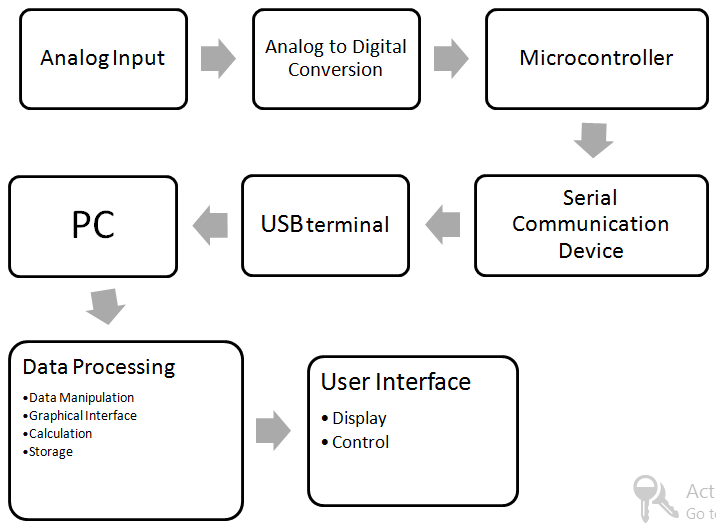
\includegraphics[scale=.5]{./Image/blockdiagram1.PNG}

\section{Advantages}
\begin{enumerate}
\item \textbf{Availability} : The major advantage of USB oscilloscope is that it can be easily available at a given place.
\item\textbf{Easily Affordable} : Even though culminating science and technology, modern day oscilloscope is far from reach of ordinary people. In this context, a USB oscilloscope would facilitate the interested ones to study the time varying signals just with the help of a PC.
\item\textbf{Portability} : It is not quite possible to carry a cathode ray oscilloscope easily. A USB oscilloscope is just a small aid box which will facilitate the user to carry it easily. It is no longer necessary to wait and find a electronics lab just to view the waveform of a time varying signal.

\end{enumerate}

\section{Limitation}
There is fundamental limit imposed on our system that can't be eliminated at all. For example the bandwidth of the system is limited by the sampling frequency which is limited by speed of ADC used. And the no of bits of ADC limits the range of the amplitude of input signal.\\

As per our preliminary calculations the bandwidth of the Oscilloscope would be $100$KHz.  And the amplitude would be limited by the no. of bits.\\

To eliminate these limitation theoretically the no. of bits should be infinite which is not practically achievable.


\begin{thebibliography}{99}
\bibitem{} Wikipedia the open internet library \emph{http://en.wikipedia.org/Oscilloscope}
\bibitem{} \emph{codeandlife.com/VUsb}
\bibitem{} Alexon, J. USB Complete: The Developer’s Guide, Fourth Edition. Lakeview Research LLC, 5310 Chinook Ln., Madison  (1999).

\end{thebibliography}

\end{document}